\documentclass{beamer}
%\usepackage{split}

\usepackage{amsmath}
\usepackage{amsfonts}
\usepackage{braket}
\usepackage{subcaption}
\usepackage{tikz}
\usepackage{xcolor}
\usetikzlibrary{positioning,shapes,arrows.meta}
%\usetikzlibrary{positioning,fit,backgrounds}
\usepackage{quantikz}
\usepackage[linesnumbered]{algorithm2e}
\usepackage{hyperref}
%\usepackage{hyperref,xcolor}
%\usepackage[ocgcolorlinks]{ocgx2}
\usepackage{cleveref}
\usepackage[backend=biber,style=authoryear,sorting=ynt]{biblatex}
\addbibresource{./sample.bib}


\newcommand*{\QACze}{ \mathbf{QAC}_{0} }
\newcommand*{\QNCzef}{ \mathbf{QNC}_{0,f} }
\newcommand*{\QNCze}{ \mathbf{QNC}_{0} }
\newcommand*{\QNCon}{ \mathbf{QNC}_{1} }
\newcommand*{\NCon}{ \mathbf{NC}_{1} }
\newcommand*{\noiseQNCon}{ noisy-$\QNCon$ }
\newcommand*{\QNC}{ \mathbf{QNC} }
\newcommand*{\QNCG}{ \mathbf{QNC_G} }
\newcommand*{\NC}{\mathbf{NC}}
\newcommand*{\QNCiG}{\mathbf{QNC_{G,i}}}


\begin{document} 

\newcommand*{\Tr}{\textbf{Tr }}


\begin{frame}
  \title{ Localitiy of Small-Set-Flip Decoder.  }
    \author{David Ponarovsky}
    \date{\today}
    \titlepage
\end{frame}


\begin{frame}

\frametitle{Introduction}

\begin{block}{Last Time:}
\begin{itemize}
  \item Quantum Expanders + orignial fault tolerance gives an almost  $\QNCon =$ \noiseQNCon. 
  \item Michael: Error decomposition into clustering happens in any LDPC code + local decoder that achieves error reduction w.h.p. exists for the $4D$-toric.
  \item Dorit: The error reduction statement should be checked, particularly, what's the structure of such a lemma when the decoding circuit is subjected to noise.

\end{itemize}
\end{block}


\begin{block}{Today:}
\begin{itemize}
  \item More about Noise, $p$-local noise $\leftrightarrow$\footnote{When using the LDPC codes} $(p^\prime, q^\prime)$-initial error per correction cycle. 
  \item  Formal statement, of the decoding theroem. 
  \item A bit on the locality of the algorithem.  
\end{itemize}
\end{block}
%\begin{block}{TAKEAWAYS:}
%\begin{itemize}
  %\item More about codes.
  %\item  First view to fault tolerance.  
  %\item Nice open problems. 
%\end{itemize}
%\end{block}
\end{frame}



\begin{frame}
  \frametitle{Nosiy Circuit.}

\begin{quantikz}[row sep=0.3cm, column sep=0.7cm]
\lstick{$q_1$} & \gate[wires=8]{U_0} & \gate{\mathcal{N}} & \gate[wires=8]{U_1}   & \gate{\mathcal{N}} & \gate[wires=8]{U_2} & \gate{\mathcal{N}}& \qw \\
\lstick{$q_2$} &                      & \gate{\mathcal{N}} &                      & \gate{\mathcal{N}} &                     & \gate{\mathcal{N}} & \qw \\
\lstick{$q_3$} &                      & \gate{\mathcal{N}} &                      & \gate{\mathcal{N}} &                     & \gate{\mathcal{N}} & \qw \\
\lstick{$q_4$} &                      & \gate{\mathcal{N}} &                      & \gate{\mathcal{N}} &                     & \gate{\mathcal{N}} & \qw \\
\lstick{$q_5$} &                      & \gate{\mathcal{N}} &                      & \gate{\mathcal{N}} &                     & \gate{\mathcal{N}} & \qw \\
\lstick{$q_6$} &                      & \gate{\mathcal{N}} &                      & \gate{\mathcal{N}} &                     & \gate{\mathcal{N}} & \qw \\
\lstick{$q_7$} &                      & \gate{\mathcal{N}} &                      & \gate{\mathcal{N}} &                     & \gate{\mathcal{N}} & \qw \\
\lstick{$q_8$} &                      & \gate{\mathcal{N}} &                      & \gate{\mathcal{N}} &                     & \gate{\mathcal{N}} & \qw
\end{quantikz}
\end{frame}




\begin{frame}{ $(p^\prime, q)$-Simplified Model. }
  \begin{definition}[Local Stochastic Noise.]
Denote by $E$ the subset of faulty qubits. We say that an error model behaves according to the local stochastic noise if:  
\begin{equation*}
  \begin{split}
    \mathbf{Pr}[|E| = t ] \le O(p^{t}) 
  \end{split}
\end{equation*}
for some $p \in (0,1)$. For example, a depolarizing channel is a local stochastic noise.
  \end{definition}
  \begin{definition}
    Let $p^{\prime}, q \in (0,1)$ and let $C$ be an error correction code. The decoding problem in the \textbf{$(p^\prime, q)$-Simplified Model} is defined as finding (a correction to) error $E$, promised the qubits are subjected to local stochastic noise $p$, and given syndrome measurement subjected to local stochastic noise $q$. We will denote by $D$ the faulty syndrome bits. 
  \end{definition}
\end{frame}

\begin{frame}{$(p^\prime, q)$-Simplified Model.}
  \begin{block}{Claim.}
    Assume that $C$ is an LDPC code, and let $D$ be a decoding algorithm which first measures the syndrome and then decode (guess a correction).  \ ~\\
Then, for any $p \in (0,1)$, there are $p^{\prime}, q \in (0,1)$ (functions of $p$ and the 'locality'\footnote{degree in the Tanner graph of $C$.} of $C$) such that the running of $D$ according to the standard $p$-noise is equivalent to its running when subjected to the $(p^{\prime}, q)$-Simplified Model. [gottesman2014]
  \end{block}
  
\end{frame}

\begin{frame}
  \begin{figure}[h]
    \begin{subfigure}[h]{0.4\textwidth}

    \label{alg:three}
    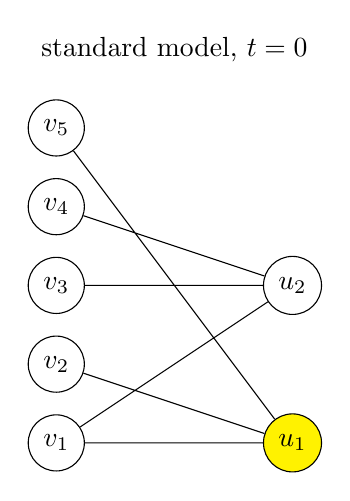
\begin{tikzpicture}%[scale=2.5]
      \draw node at (1.5,6) {standard model, $t =0$};
\tikzstyle{every node}=[draw,shape=circle];

\draw node[fill=yellow] (v0) at (3,1) {$u_1$};
\draw node (v6) at (3,3) {$u_2$};
\draw node foreach \x in {1,2,3,4,5} (v\x) at (0,\x) {$v_\x$};

\draw (v0) -- (v1)
(v0) -- (v2)
(v0) -- (v5)
(v6) -- (v3)
(v6) -- (v4)
(v6) -- (v1);
\end{tikzpicture}
    \end{subfigure}
    \begin{subfigure}[h]{0.1\textwidth}
      \
    \end{subfigure}
    \begin{subfigure}[h]{0.45\textwidth} 

    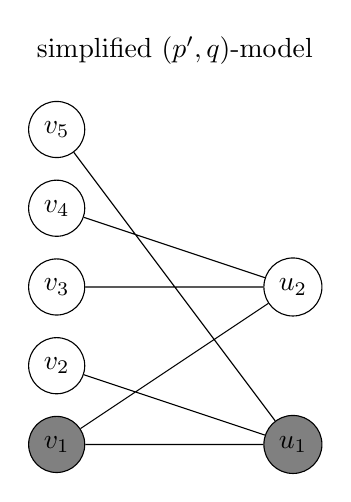
\begin{tikzpicture}%[scale=2.5]
      \draw node at (1.5,6) { simplified $(p^{\prime},q)$-model};
\tikzstyle{every node}=[draw,shape=circle];

\draw node[fill=gray] (v0) at (3,1) {$u_1$};
\draw node (v6) at (3,3) {$u_2$};
\draw node foreach \x in {2,3,4,5} (v\x) at (0,\x) {$v_\x$};
\draw node[fill=gray] (v1) at (0,1) {$v_1$};
\draw (v0) -- (v1)
(v0) -- (v2)
(v0) -- (v5)
(v6) -- (v3)
(v6) -- (v4)
(v6) -- (v1);
\end{tikzpicture}
    \label{fig:location}
    \end{subfigure} 
  \end{figure}

\end{frame}

\begin{frame}
  \begin{figure}[h]
    \begin{subfigure}[h]{0.4\textwidth}

    \label{alg:three}
    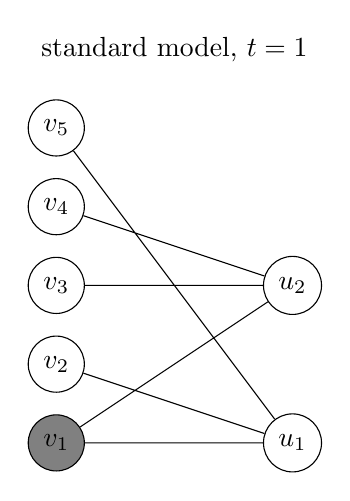
\begin{tikzpicture}%[scale=2.5]
      \draw node at (1.5,6) {standard model, $t =1$};
\tikzstyle{every node}=[draw,shape=circle];

\draw node (v0) at (3,1) {$u_1$};
\draw node (v6) at (3,3) {$u_2$};
\draw node foreach \x in {2,3,4,5} (v\x) at (0,\x) {$v_\x$};
\draw node[fill=gray] (v1) at (0,1) {$v_{1}$};
\draw (v0) -- (v1)
(v0) -- (v2)
(v0) -- (v5)
(v6) -- (v3)
(v6) -- (v4)
(v6) -- (v1);
\end{tikzpicture}
    \end{subfigure}
    \begin{subfigure}[h]{0.1\textwidth}
      \
    \end{subfigure}
    \begin{subfigure}[h]{0.45\textwidth} 

    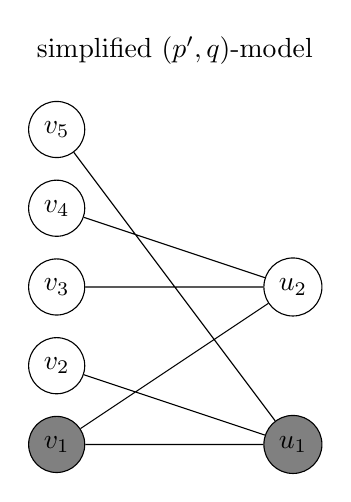
\begin{tikzpicture}%[scale=2.5]
      \draw node at (1.5,6) {simplified $(p^{\prime},q)$-model};
\tikzstyle{every node}=[draw,shape=circle];

\draw node[fill=gray] (v0) at (3,1) {$u_1$};
\draw node (v6) at (3,3) {$u_2$};
\draw node foreach \x in {2,3,4,5} (v\x) at (0,\x) {$v_\x$};
\draw node[fill=gray] (v1) at (0,1) {$v_1$};
\draw (v0) -- (v1)
(v0) -- (v2)
(v0) -- (v5)
(v6) -- (v3)
(v6) -- (v4)
(v6) -- (v1);
\end{tikzpicture}
    \label{fig:location}
    \end{subfigure} 
  \end{figure}

\end{frame}
\begin{frame}
  \begin{figure}[h]
    \begin{subfigure}[h]{0.4\textwidth}

    \label{alg:three}
    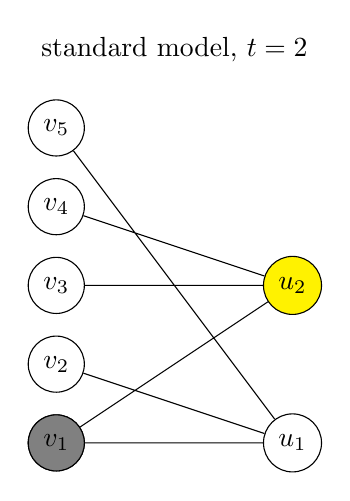
\begin{tikzpicture}%[scale=2.5]
      \draw node at (1.5,6) {standard model, $t =2$};
\tikzstyle{every node}=[draw,shape=circle];

\draw node (v0) at (3,1) {$u_1$};
\draw node[fill=yellow] (v6) at (3,3) {$u_2$};
\draw node foreach \x in {1,2,3,4,5} (v\x) at (0,\x) {$v_\x$};
\draw node[fill=gray] (v1) at (0,1) {$v_{1}$};
\draw (v0) -- (v1)
(v0) -- (v2)
(v0) -- (v5)
(v6) -- (v3)
(v6) -- (v4)
(v6) -- (v1);
\end{tikzpicture}
    \end{subfigure}
    \begin{subfigure}[h]{0.1\textwidth}
      \
    \end{subfigure}
    \begin{subfigure}[h]{0.45\textwidth} 

    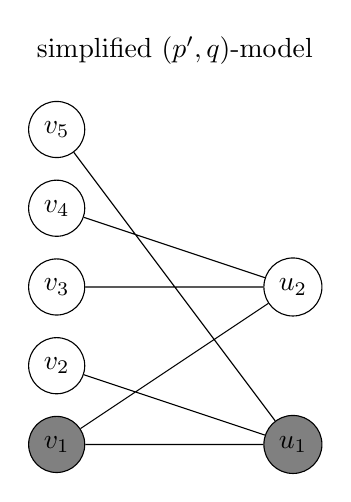
\begin{tikzpicture}%[scale=2.5]
      \draw node at (1.5,6) {simplified $(p^{\prime},q)$-model};
\tikzstyle{every node}=[draw,shape=circle];

\draw node[fill=gray] (v0) at (3,1) {$u_1$};
\draw node (v6) at (3,3) {$u_2$};
\draw node foreach \x in {2,3,4,5} (v\x) at (0,\x) {$v_\x$};
\draw node[fill=gray] (v1) at (0,1) {$v_1$};
\draw (v0) -- (v1)
(v0) -- (v2)
(v0) -- (v5)
(v6) -- (v3)
(v6) -- (v4)
(v6) -- (v1);
\end{tikzpicture}
    \label{fig:location}
    \end{subfigure} 
  \end{figure}

\end{frame}

\begin{frame}{Reducing error formal statement.}
\begin{figure}[h]
    \centering
    \includegraphics[width=\textwidth]{formal_state_ment_error_reduction.png}
    \caption{ Formal statement, error reduction using the Small-set-flip parallel decoder.}
    \label{fig:your-label}
\end{figure}

\end{frame}



\begin{frame}
  \begin{block}{Decoder. (Simplified version).}
    Look for a 'small set' $F$ of qubits such that:
    \begin{enumerate}
      \item $F$ contained in the support of some $X$-type stabilizer. 
      \item $F$ toched many unstaisfied $Z$-type stabilizer. Or, flipping $F$, decrease the $Z$-type syndrom.    
    \end{enumerate}
  \end{block}
For parallelizing the decoder, we color the check nodes in the Tanner graph such that no two checks of the same color share a bit.\footnote{Since the code is LDPC, we can do it with $O(1)$ colors.} Then, in the $i$th iteration, we look in parallel over all $X$-type stabilizers at the $i$th color.
\end{frame}


\begin{frame}{Locality.}

  \begin{block}
Denote by $U = E \cup F_1 \cup F_2, \ldots, F_m$ the execution support, the combination of faulty qubits and the qubits flipped by the decoder.
  \end{block}

  \begin{block}
  For any set $K\subset U$ with $\Gamma_{Q}(K)\cap \Gamma_{Q}(U / K) = \emptyset$ there is a valid executation of the Decoder, on the input $(E \cap K, D\cap \Gamma_{X}(K))$ whose output is $\hat{E}\cap K$ and whose support is $U \cap K$.
\end{block} \footnote{
An execution might change upon the order of the small set being chosen, yet notice that for small errors, the algorithm is always correct.
}
\end{frame}

\newcommand*{\MC}{ \text{MaxConn}_\alpha }
\begin{frame}
  \begin{definition}{$\alpha$-subset, and $\MC$. (Simplified\footnote{In the original, the graph is the syndorm graph}) } 
    Let $G$ be a graph. Let $X,Y \subset \mathcal{V}$ and $\alpha \in (0,1]$. $X$ is said to be an $\alpha$-subset of $Y$ if $|X \cap Y| \ge \alpha |X|$. In addition we define: 
    
    \begin{equation*}
      \begin{split}
        \MC(Y) = \max{ \{ |X| :  X \text{ is connected in  } G \text{ and is an } \alpha \text{ subset of } Y \} }
      \end{split}
    \end{equation*}
  \end{definition}

Notice that if $X$ is an $\alpha$-subset of $Y$ then: 
\begin{equation*}
  \begin{split}
    |X| \le \frac{1}{\alpha} |Y| 
  \end{split}
\end{equation*}

\end{frame}



\begin{frame}

\begin{figure}[h]
    \centering
    \includegraphics[width=\textwidth]{preculation.png}
    \caption{ Formal statement, error reduction using the Small-set-flip parallel decoder.}
    \label{fig:your-label}
\end{figure}

So with probability $1 - e^{\sqrt{n}}$ we have that $\MC(E) < \gamma \sqrt{n}$.  

\end{frame}



\begin{frame}{The Decoding Algorithm.}
  First noitce that the repetition code could be defined as Tanner code, for any $\Delta$-regular graph $G$ and local code $C_{0}$ which is the repetition over $\Delta$ bits.   


  In particular $G$ could be a bipartite expander graph. Denote the right and the left vertices subsets by $V^{-}$ and $V^{+}$.
  \begin{block}{Decoding:}
    For $\Omega\left( \log n \right)$ iterations, do: 
  \begin{enumerate}
    \item In every even iteration, all the vertices in $V^{+}$ 'correct' their local view based on the majority.
    \item In every odd iteration, all the vertices in $V^{-}$ 'correct' their local view based on the majority.
  \end{enumerate}
For having a constant depth error reduction procedure, it's enough to run the decoding above for two iterations.
\end{block}

\end{frame}


\begin{frame}{The Decoding Algorithm.}

  
  \begin{figure}[h]
    \begin{subfigure}[h]{0.4\textwidth}

    \label{alg:three}
      \begin{algorithm}[H]
    \KwData{ $x \in \mathbb{F}_{2}^{n}$ }
    \For { $ v \in V^{+}$} {
      $x^{\prime}_{v} \leftarrow \arg\min {\left\{  y \in C_{0} : |y + x|_{v} |  \right\} } $\\
    }
    \For { $ v \in V^{-}$} {
      $x^{\prime}_{v} \leftarrow \arg\min {\left\{  y \in C_{0} : |y + x|_{v} |  \right\} } $\\
    }
    \Return  $x $

  \end{algorithm}
    \end{subfigure}
    \begin{subfigure}[h]{0.1\textwidth}
      \
    \end{subfigure}
    \begin{subfigure}[h]{0.45\textwidth} 

    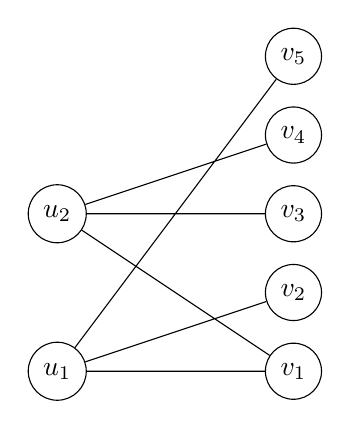
\begin{tikzpicture}%[scale=2.5]
\tikzstyle{every node}=[draw,shape=circle];

\draw node (v0) at (0,1) {$u_1$};
\draw node (v6) at (0,3) {$u_2$};
\draw node foreach \x in {1,2,3,4,5} (v\x) at (3,\x) {$v_\x$};

\draw (v0) -- (v1)
(v0) -- (v2)
(v0) -- (v5)
(v6) -- (v3)
(v6) -- (v4)
(v6) -- (v1);
\end{tikzpicture}
    \label{fig:location}
    \end{subfigure} 
  \end{figure}

\end{frame}

\begin{frame}{The Decoding Algorithm.}
  \begin{block}{Proof.}
  Denote by $S^{(0)} \subset V^{+}$ and  $T^{(0)} \subset V^{-}$ the subsets of left and right vertices adjacent to the error. And denote by $T^{(1)} \subset T^{(0)}$ the right vertices such any of them is connect by at least $\frac{1}{2}\Delta$ edges to vertices at $S^{(0)}$. \\~\

  Note that that any vertex in $V^{-}/T^{(1)}$ has on his local view less than $\frac{1}{2}\Delta$ faulty bits, So it corrects into his 'right' (codeword in $C_{0}$) local view in the first right correction round. \\~\

  Therefore after the right correction round the error is set only on $T^{(1)}$'s neighbourhood, namely at size at most $\Delta|T^{(1)}|$. We will show:
  \begin{equation*}
    \begin{split}
  \Delta|T^{(1)}| \le \text{constant} \cdot |e|
    \end{split}
  \end{equation*}
\end{block}
\end{frame}
\begin{frame}

  Using the expansion property we get an upper bound on $T^{(1)}$ size: \begin{equation*}
  \begin{split} 
    \frac{1}{2}\Delta |T^{(1)}| & \le \Delta \frac{|T^{(1)}||S^{(0)}|}{n} + \lambda\sqrt{|T^{(1)}||S^{(0)}|} \\ 
  \left( \frac{1}{2}  \Delta - \frac{|S^{(0)}|}{n} \Delta \right) |T^{(1)}| & \le \lambda \sqrt{|T^{(1)}||S^{(0)}|} \\ 
  \Delta^{2}|T^{(1)}| & \le \left( \frac{1}{2}  - \frac{|S^{(0)}|}{n}  \right)^{-2}\lambda^{2} |S^{(0)}| 
  \end{split}
\end{equation*}
Since any left vertex adjoins to at least single faulty bit we have that $|S^{(0)}| \le |e|$. Combing with the inequality above we get:  

\begin{equation*}
  \begin{split}
    \Delta |T^{(1)}| \le \left( \frac{1}{2}   - \frac{|e|}{n} \right)^{-2}\lambda^{2} \frac{|e|}{\Delta}
  \end{split}
\end{equation*}
Hence for $|e|/n \le \beta =  \frac{1}{2}   - \sqrt{\frac{2\lambda^{2}}{\Delta}}$ it holds that $\Delta|T^{(1)}| \le \frac{1}{2}|e|$. \footnote{Reminder for David!!! Explain why $\lambda^2/\Delta \ge 1 $, and to describe how to correct the proof.}




\end{frame}




\begin{frame}
  \frametitle{The Franch's Construction.
}

  \begin{refsection}
\cite{Tillich_2014} \cite{Leverrier_2015} \cite{grospellier:tel-03364419}
  \printbibliography
\end{refsection}

\end{frame}


\begin{frame}{The Franch's Construction.}
 \begin{block}{Franch gadgets.}
   \begin{itemize}
     \item Encoded states and magic preparation (via original fault tolerance).
     \item Hypergraph product code. (Quantum Expander Codes). $\left[ \left[ n, \Theta(n), \Theta(\sqrt{n}) \right] \right]$.
   \end{itemize}
 \end{block}
\end{frame}

\begin{frame}
  \begin{block}{Theorem \footnote{Theorem 6.4 in \cite{grospellier:tel-03364419}}} There exists a threshold $p_{0}$ such that the following holds. Let $p < p_{0}$, let $\delta > 0$ and let $D$ be a circuit with $m$ qubits, with $T$ time steps and $|D|$ locations. We assume that the output of $D$ is a quantum state $\ket{\psi}$. 

    Then there exists another circuit $D^{\prime}$ whose output is $\ket{\psi}$ and such that when $D^{\prime}$ is subjected to a local noise model with parameter $p$, there exists a $\mathcal{N}$ a local stochastic noise on the qubits of $\ket{\psi}$ with parameters $p^{\prime} = c \cdot p$ such that: 

    \begin{equation*}
      \begin{split}
        \mathbf{Pr}[  \text{ output of } D^{\prime} \text { is not } \mathcal{N}\left( \ket{\psi} \right)   ]\le \delta
      \end{split}
    \end{equation*}
    In addition $D^{\prime}$ has $m^{\prime}$ qubits and $T^{\prime}$ time steps where: 

    \begin{equation*}
      \begin{split}
        m^{\prime} &= m \text{ polylog } \left( |D|/\delta \right) \\ 
        T^{\prime} &= T \text{ polylog } \left( |D|/\delta \right) 
      \end{split}
    \end{equation*}
  \end{block}
\end{frame}


\begin{frame}{Proof Sketch.}

  \scalebox{0.8}{
\begin{quantikz}%[row sep=0.3cm, column sep=0.7cm]
  \lstick{$q_1$} & \gate[wires=9][1.7cm]{\Phi^{k}(D)} & \gate{\mathcal{N}} &   \gate[wires=3]{\Phi^{k-1}(\mathcal{E}^{-1})} & \gate{\mathcal{N}} & \gate[wires=2]{\Phi^{k-2}(\mathcal{E}^{-1})}   & \gate{\mathcal{N}} & \qw &\\
  \lstick{$q_2$} &                      & \gate{\mathcal{N}} &                & \gate{\mathcal{N}} &                      & \gate{\mathcal{N}} & \qw &\\
  \lstick{$q_3$} &                      & \gate{\mathcal{N}} &                & \gate{\mathcal{N}} &                      & \gate{\mathcal{N}} & \qw &\\
  \lstick{$q_4$} &                      & \gate{\mathcal{N}} &     \gate[wires=3]{\Phi^{k-1}(\mathcal{E}^{-1})} & \gate{\mathcal{N}} & \gate[wires=2]{\Phi^{k-2}(\mathcal{E}^{-1})}                                 & \gate{\mathcal{N}} & \qw &\\
  \lstick{$q_5$} &                      & \gate{\mathcal{N}} &                & \gate{\mathcal{N}} &                      & \gate{\mathcal{N}} & \qw &\\
  \lstick{$q_6$} &                      & \gate{\mathcal{N}} &                & \gate{\mathcal{N}} &                      & \gate{\mathcal{N}} & \qw &\\
  \lstick{$q_7$} &                      & \gate{\mathcal{N}} &      \gate[wires=3]{\Phi^{k-1}(\mathcal{E}^{-1})} & \gate{\mathcal{N}} & \gate[wires=2]{\Phi^{k-2}(\mathcal{E}^{-1})}                                & \gate{\mathcal{N}} & \qw &\\
  \lstick{$q_8$} &                      & \gate{\mathcal{N}} &                & \gate{\mathcal{N}} &                      & \gate{\mathcal{N}} & \qw &\\
  \lstick{$q_9$} &                      & \gate{\mathcal{N}} &                & \gate{\mathcal{N}} &                      & \gate{\mathcal{N}} & \qw &
\end{quantikz}
}


\end{frame}

\begin{frame}{Proof Sketch.}

The probability that the $i$th bit will absorb an error at the end is bounded by:
  \begin{equation*}
    \begin{split}
      \left( cp \right)^{2^{k-1}} + \left( cp \right)^{2^{k-2}} + .. \left( cp \right)^{2^{k-3}} + .. +  cp \le c_{2}p 
    \end{split}
  \end{equation*}
So we prepared the state $\ket{\psi}$, subjected to local noise (depolarizing noise) at rate $c_{2}p$. \\~\

\begin{block}{Corollary}
  We can assume that we have an accsess to polynomialy number of magic states encoded in whatever code we like.
  Moreover, denote by $n$ the complexitiy parameter (input length). if the encoding gate (of the desired code) is $D$ and it's depth is $T$, such that 
  \begin{equation*}
    \begin{split}
      T \mathbf{poly log} \left( |D| \right) = O(\log n)
    \end{split}
  \end{equation*}
  then the preparation of the magic is in\noiseQNCon.
\end{block}

\end{frame}

\begin{frame}
  \frametitle{Hypergraph Product Code.}
\begin{figure}[h]
    \centering
    \includegraphics[width=\textwidth]{Hypergraph_prod.png}
    \caption{ Hypergraph Product code Tanner graph / stabilizers. }
    \label{fig:your-label}
\end{figure}

\end{frame}

\begin{frame}
  \frametitle{Hypergraph Product Code.}

\begin{figure}[h]
    \centering
    \includegraphics[width=0.8\textwidth]{toric_prod.png}
    \caption{The Toric code can be thought of as the hypergraph product obtained by multiplying the repetition code with itself.}
    \label{fig:your-label}
\end{figure}

\end{frame}

\begin{frame}{Error reduction in the Quantum Expander Code.}
  \begin{block}{Quantum Expander Code.}
    Consider $C_{1},C_{2}$ (classical) expanders codes\footnote{such $C_{1}^{\perp}, C_{2}^{\perp}$ also have a good distance.}. Consider the Hypergraph code defined by them.
  \end{block}


  \begin{block}{Proof Idea}
    \begin{itemize}
      \item First, proving that for adversarial errors with weight at most $\alpha \sqrt{n}$, the error can be reduced by a constant factor. The proof uses the expansion in classical codes.
      \item Second, showing that with probability $1 - \Theta(e^{-\sqrt{n}})$, the error can be decomposed into disjoint errors, each with a size of at most $\alpha \sqrt{n}$.
    \end{itemize}
\end{block}
\end{frame}


\begin{frame}
  \frametitle{Fault Tolerance at Constant Space Overhead.}

  \begin{block}{Start.}
    We preapere $\sqrt{n}$ blocks at length $\Theta(\sqrt{n})$ each, we do it sesenqutaly, so the preaperation requires $\Theta(\sqrt{n} \mathbf{ poly log} n)$ anciles. 
  \end{block}
 
  \begin{block}{Error reduction.}
Constantly apply rounds of error reduction.
  \end{block}
  \begin{block}{Simulate a gate.}
    \begin{itemize}
      \item  If the gate is a logical Pauli, we apply it in a transversal manner.
      \item We prepare the magic state suite for the gate and simulate the gate using the magic procedure - Entangle the states (through transversal CNOT), measure and decode the measurement. 

        Then applying a correction which might be either transversal logical Pauli (if the gate were Clifford) or logical Clifford (if the gate were T). For the second we will have to reapet on the procedure. 
    \end{itemize}
  \end{block}


\end{frame}

\begin{frame}{Fault Tolerance at Constant Space Overhead.}
\begin{figure}[h]
    \centering
    \includegraphics[width=\textwidth]{magic_prod.png}
    \label{fig:your-label}
\end{figure}
\end{frame}

\begin{frame}{An almost $\QNCon =$ \noiseQNCon}
  Encode each qubit by exapnder code at length $\Theta(\log^{10}(n))$. Prepere $2|D|$ magic states form each type in the beginning. \\~\ 

Where did we cheat? \\~\

Decide what correction to apply $UPU^{\dagger}$ given the measurement is not a trivial task. In particular, it isn't clear if it can be done in constant depth.
\end{frame}


\begin{frame}{Open Problems.}
  \begin{itemize}
    \item Is there a non-trivial lower bound for deciding $UPU^{\dagger}$?
    \item Implementing logical gates natively without magic states at a constant depth.
  \end{itemize}
\end{frame}


\begin{frame}{Sheets.}
  \begin{enumerate}
    \item The Tanner graph of the classical code $C_{X}$ used to correct $X$-type errors is the subgraph of $G_{Q}$ induced by the $V \times V \cup C \times C$ qubits and the set of $Z$-type generators.  
  \end{enumerate}
\end{frame}

\end{document}
